\documentclass[a4paper,12pt]{article}
\usepackage[bahasa]{babel}
\usepackage{graphicx}
\usepackage{multirow}
\usepackage{enumitem}
\usepackage{listings}
\usepackage{adjustbox}
\graphicspath{ {./img/} }
\begin{document}
\title{Laporan Praktikum Statistika Pertemuan 12}
%\author{Aldzikri Dwijayanto Prathama \\ {\small 195410189}}
\author{Aldzikri Dwijayanto Prathama 
	\\195410189}
\makeatletter
\begin{titlepage}
	\begin{center}
		{\huge \bfseries \@title }\\[14ex]
		
\includegraphics[scale=.8]{logo}\\[4ex]
		{\large \@author}\\[20ex]
		{\large \bfseries {SEKOLAH TINGGI MANAJEMEN INFORMATIKA DAN KOMPUTER
				AKAKOM YOGYAKARTA}}
	\end{center}


%{\large \@date} 
\end{titlepage}
\makeatother
%\maketitle
\newpage
\tableofcontents
\newpage
\section{Pembahasan}
\begin{enumerate}[label=\textbf{\Alph*}.]
    \item \textbf{DISTRIBUSI NORMAL}\\
	Distribusi normal, disebut juga distribusi Gauss, adalah distribusi probabilitas yang paling banyak digunakan dalam berbagai analisis statistika dan kebanyakan pengujian hipotesis mengasumsikan normalisasi suatu data. 
    Distribusi normal baku adalah distribusi normal yang memiliki rata-rata nol dan simpangan baku satu. Distribusi ini juga dijuluki kurva lonceng (bell curve) karena grafik fungsi kepekatan probabilitasnya mirip dengan bentuk lonceng. Distribusi normal memiliki sifat simetris, yaitu mean distribusi terletak di tengah dengan luas bagian sebelah kiri sama dengan bagian sebelah kanan (berbentuk lonceng) sehingga total daerah di bawah kurva sebelah kiri = total daerah di bawah kurva sebelah kanan = 0,5	
    \item \textbf{DISTRIBUSI STUDENT'S t}\\
	Distribusi student’s t adalah distribusi yang ditemukan oleh seorang mahasiswa yang tidak mau disebut namanya. Untuk menghargai hasil penemuannya itu, distribusinya disebut distribusi Student yang lebih dikenal dengan distribusi “t”, diambil daru huruf terakhir kata “student”
\end{enumerate}
\newpage
\section{Praktik}
\begin{enumerate}[label=\textbf{\Alph*.}]
	\item Menghitung probabilitas  data berdistribusi Normal
	\paragraph{Praktik 1\\}
Apabila X berdistribusi Normal dengan rata-rata 3 dan standar deviasi 0.5, tentukan probabilitas

\begin{enumerate}[label=\alph*.]
  \item $P(X = 4)$\\
  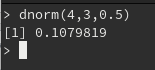
\includegraphics[scale=1]{praka1a}\\
  Diketahui:
  \begin{itemize}
  	\item X = 4
  	\item mean = 3
  	\item sd = 0.5
  \end{itemize}
  Pada soal a adalah mencari probabiliatas kumulatif x dengan rata-rata $\lambda$
  Atau P(X = x), sehingga kita gunakan perintah dnorm, format dari perintah dnorm adalah seperti berikut\\
  \texttt{>dnorm(x, mean, sd)\\}
  Jadi untuk soal ini perintahnya adalah\\
  \texttt{dnorm(4,3,0.5)}\\
  Dari output di atas diketahui bahwa $P(X = 4) = 0,10798$
  
  \item $P (X < 3,5)$\\
  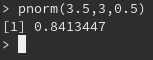
\includegraphics[scale=1]{praka1b}\\
  Diketahui:
  \begin{itemize}
  	\item X < 3.5
  	\item mean = 3
  	\item sd = 0.5
  \end{itemize}
  Pada soal b adalah mencari probabiliatas kumulatif x  dengan rata-rata $\lambda$
  Atau $P(X < x)$, sehingga kita gunakan perintah pnorm, format dari perintah dnorm adalah seperti berikut\\
  \texttt{>pnorm(x, mean, sd)\\}
  Jadi untuk soal ini perintahnya adalah\\
  \texttt{pnorm(3.5,3,0.5)}\\
  Dari output di atas diketahui bahwa $P(X < 4) = 0,841$
\end{enumerate}

\paragraph{Praktik 2\\}
Apabila X berdistribusi Normal dengan rata-rata 10 dan standar deviasi 0.65, tentukan probabilitas 
\begin{enumerate}
	\item $P(3 < X < 7)$\\
	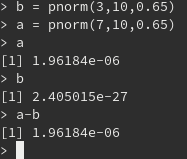
\includegraphics{praka2a}\\
	Diketahui:
	\begin{itemize}
		\item mean = 10
		\item sd = 0.65 
		\item $P(3 < X < 7) = P(X < 7) - P(X < 3)$ 
	\end{itemize}
	Pada soal ini adalah mencari probabiliatas kumulatif x  dengan rata-rata $\lambda$
	Atau $P(X < x)$, sehingga kita gunakan perintah pnorm.
	Untuk penyelesaiannya pertama kita cari $P(X < 3)$\\
	\texttt{b = pnorm(3,10,0.65)}\\
	lalu cari $P(X < 7)$\\
	\texttt{a = pnorm(7,10,0.65)}\\
	lalu kurangi $P(X < 7)$ dengan $P(X < 3)$
	\texttt{a-b}\\
	dari hasil di atas diketahui $P(3 < X < 7) = 1,9610^{-6}$

    \item $P(X \geq 3)$\\
        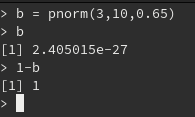
\includegraphics{praka2b}\\
        Diketahui:
        \begin{itemize}
            \item mean = 10
            \item sd = 0.65 
            \item $P(X \geq 3) = 1 - P(X < 3)$ 
        \end{itemize} 
        Pada praktik ini digunakan perintah \texttt{pnorm} karena akan dicari $P(X < 3)$\\
        \texttt{b = pnorm(3,10,0.65)}\\
        Lalu kurangi 1 dengan hasil operasi tadi\\
        \texttt{1-b}\\
        Dari output diatas diketahui $P(X \geq 3) = 1$ 

\end{enumerate}

\item Membangkitkan data berdistribusi Normal\\
    Akan digenerate data berdistribusi normal dengan jumlah data 30, mean = 0 dan sd =1.\\
    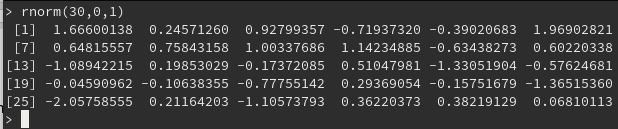
\includegraphics[scale=.7]{prakb}\\
    Untuk membangkitkan n data berdidtribusi normal dengan parameter mean dan sd gunakan perintah\\
    \texttt{rnorm(n, mean, sd)}\\
    Untuk membangkitkan data berdistribusi normal dengan jumlah data 30, mean = 0, dan sd = 1 perintahnya adalah\\
    \texttt{rnorm(30,0,1)}

\item Menghitung nilai x yang membatasi luas daerah(nilai peluang) distribusi Normal\\
    \paragraph{Praktik 1\\}
    Tentukan nilai kritis z dimana P(Z < z) = 0,95\\
    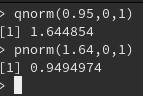
\includegraphics{prakc1}\\
    Diketahui:     mencari probabiliatas kumulatif x  dengan derajat kebebasan df
 Atau P(X < x)
    \begin{itemize}
        \item P = 0.95
        \item mean = 0  
        \item sd = 1
    \end{itemize}
    Untuk mencari nilai x dari luasan (peluang) P berdistribusi Normal dengan parameter mean dan sd gunakan perintah \texttt{qnorm}
    \texttt{qnorm(0.95,0,1)}\\
        Jadi diketahui $P(Z < z) = 0,95 maka z = 1,64$

    \paragraph{Praktik 2\\}
    Tentukan nilai kritis x dimana P(X < x) = 0,95, untuk X berdistribusi Normal dengan mean 3, standar deviasi 0.5\\
    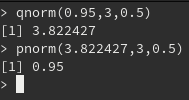
\includegraphics{prakc2}
    \begin{itemize}
        \item P = 0.95
        \item mean = 3  
        \item sd = 0.5
    \end{itemize}
    Untuk mencari nilai kritis x digunakan perintah \texttt{qnorm}\\
    \texttt{qnorm(0.95,5,0.5)}\\
    Jadi diketahui $P(X < x) = 0,95 maka x = 3,82$

\item Menghitung probabilitas  distribusi student\\
    \paragraph{Praktik 1\\}
    Hitung probabilitas distribusi t dengan nilai dengan db=9
    \begin{enumerate}[label=\alph*.]
        \item P( t = 2.5)\\
            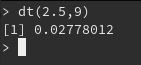
\includegraphics{prakd1a}\\
            Diketahui
            \begin{itemize}
                \item t = 2.5
                \item db = 9
            \end{itemize}
            Untuk mencari probabiliatas kumulatif x dengan derajat kebebasan df Atau P(X = x) gunakan perintah \texttt{dt}, jadi untuk soal ini perintahnya adalah\\
            \texttt{dt(2.5,9)}\\
            Jadi diketahui $P( t = 2,5) = 0,02778$

        \item $P(t < 2.5 )$\\
            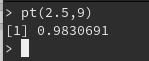
\includegraphics{prakd1b}\\
            Diketahui
            \begin{itemize}
                \item $t < 2.5$
                \item db = 9
            \end{itemize}
            Untuk mencari probabiliatas kumulatif x  dengan derajat kebebasan df Atau $P(X < x)$ gunakan perintah \texttt{pt}\\
            \texttt{pt(2.5,9)}\\
            Dari operasi tersebut diketahui $P( t <  2,5) = 0,983$

        \item $P(t > 2.5)$\\
            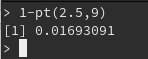
\includegraphics{prakd1c}\\
            Untuk mencari $P(t > 2.5)$ caranya adalah menguranggi 1 dengan hasil dari $P(t < 2.5)$\\
            \texttt{1-pt(2.5,9)}
            Jadi diketahui $P(t > 2.5) = 1 - P( t <  2,5) =1 -  0,983 = 0.01693091$
    \end{enumerate}

\item Membangkitkan data berdistribusi student-t\\
    Akan digenerate data berdistribusi t dengan n = 30 derajat bebas (df) = 29\\
    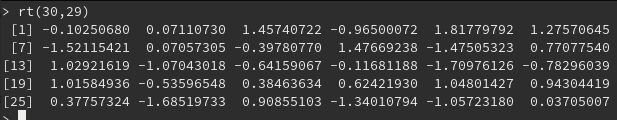
\includegraphics[scale=.7]{prake}
    Untuk membangkitkan n data berdidtribusi student’s dengan derajat kebebasan df gunakan fungsi \texttt{rt (n, df)}\\

\item Menghitung nilai x yang membatasi luas daerah(nilai peluang) distribusi Student’s\\
    Tentukan nilai kritis t dimana P(T < t) = 0,95 dengan derajat bebas 10\\
    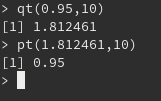
\includegraphics{prakf}
    Untuk mencari nilai x dari luasan (peluang) P berdistribusi 
     student’s dengan derajat kebebasan df gunakan perintah \texttt{qt(P, df)} 
     $P(T < t) = 0,95 maka t = 1,812461$

\end{enumerate}

\section{Latihan}
\paragraph{Latihan 1\\}
Apabila X berdistribusi Normal dengan rata-rata 10 dan standar deviasi 1.5, tentukan probabilitas
\begin{enumerate}[label=\alph*.]
    \item $P(X = 5)$\\
        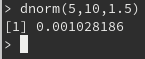
\includegraphics{lat1a}\\
        Diketahui:
        \begin{itemize}
            \item mean = 10
            \item sd = 1.5
        \end{itemize}
        Karena berdistribusi normal dan dicari $P(X = 5)$ maka gunakan perintah dnorm\\  
        Perintah:\\
        \texttt{dnorm(5,10,1.5)}
        Jadi diketahui $P(X = 5) = 0.001$

    \item $P(X < 5)$\\
        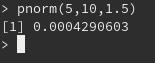
\includegraphics{lat1b}\\
        Diketahui:
        \begin{itemize}
            \item mean = 10
            \item sd = 1.5
        \end{itemize}
        Karena berdistribusi normal dan dicari $P(X < 5)$ maka gunakan perintah pnorm\\  
        Perintah:\\
        \texttt{dnorm(5,10,1.5)}
        Jadi diketahui $P(X < 5) = 0.0004$

    \item $P(5 < X < 11)$\\
        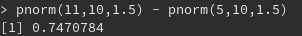
\includegraphics{lat1c}\\
        Diketahui:
        \begin{itemize}
            \item mean = 10
            \item sd = 1.5
        \end{itemize}
        Karena berdistribusi normal dan dicari $P(X < 11)$ dan $P(X < 5)$ maka gunakan perintah pnorm\\  
        Perintah:\\
        \texttt{pnorm(11,10,1.5) - pnorm(5,10,1.5)}
        Jadi diketahui $P(5 < X < 11) = 0.747$

    \item $P(X > 7)$\\
        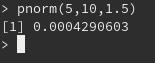
\includegraphics{lat1b}\\
        Diketahui:
        \begin{itemize}
            \item mean = 10
            \item sd = 1.5
        \end{itemize}
        Karena berdistribusi normal dan dicari $P(X > 7)$ maka gunakan perintah pnorm\\  
        Perintah:\\
        \texttt{1- pnorm(6,10,1.5)}
        Jadi diketahui $P(X > 6) = 0.996$

\end{enumerate}

\paragraph{Latihan 2\\}
Tentukan nilai kritis x dimana P(X < x) = 0,90, untuk X berdistribusi Normal dengan mean 6, standar deviasi 1.5\\
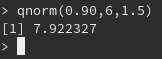
\includegraphics{lat2}\\
Diketahui:
\begin{itemize}
    \item P = 0.90
    \item mean = 6
    \item sd = 1.5
\end{itemize}
\texttt{qnorm(0.90,6,1.5)}
Hasilnya adalah 7.9

\paragraph{Latihan 3}
Apabila X berdistribusi Student’s dengan derajat bebas 10, tentukan probabilitas\\
\begin{enumerate}[label = \alph*.]
    \item P(X = 4)\\
        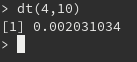
\includegraphics{lat3a}\\
        Diketahui:
        \begin{itemize}
            \item x = 4
            \item db = 10
        \end{itemize}
        Gunakan perintah dt\\
        \texttt{dt(4,10)}\\
        Diketahui $P(X = 4) = 0.002$


    \item P(X < 6)\\
        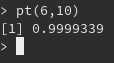
\includegraphics{lat3b}\\
        Diketahui:
        \begin{itemize}
            \item x < 6
            \item db = 10
        \end{itemize}
        Gunakan perintah pt\\
        \texttt{pt(6,10)}\\
        Diketahui $P(X < 6) = 0.9999$

    \item P(7 < X < 20)\\
        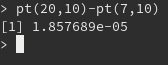
\includegraphics{lat3c}\\
        Diketahui:
        \begin{itemize}
            \item db = 10
        \end{itemize}
        Gunakan perintah pt\\
        \texttt{pt(20,10)-pt(7,10)}\\
        Diketahui $P(7 < X < 20) = 1.857$

    \item P(X > 20)\\
        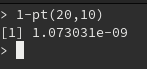
\includegraphics{lat3d}\\
        Diketahui:
        \begin{itemize}
            \item x > 20
            \item db = 10
        \end{itemize}
        Gunakan perintah pt\\
        \texttt{1-pt(20,10)}\\
        Diketahui $P(X > 20) = 1.07$

\end{enumerate}
\paragraph{Latihan 4\\}
Bangkitkan data berdistribusi t dengan n = 95, db = 94\\
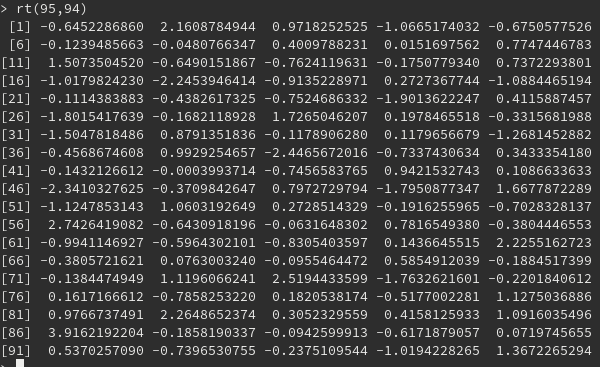
\includegraphics[scale = .7]{lat4}\\

\section{Tugas}
\paragraph{Tugas 1\\}
Jika mass sebuah bantalan peluru (ball bearing) yang diproduksi suatu pabrik memiliki distribusi normal dengan mean 0,614 kg dan deviasi standard 0,0025 kg, tentukan persentase banyaknya bantalan peluru yang memiliki massa :
\begin{enumerate}[label=\alph*.]
    \item antara 0,610 sampai 0,618 kg\\
        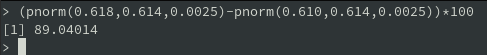
\includegraphics[width=\linewidth]{tugas1a}\\
        Pada tugas ini kita akan menentukan probabilitas jika X 0,610 sampai 0,618 maka kita gunakan 2 perintah pada Rconsole. Untuk mencari probabiliatas kumulatif x dengan rata-rata $\lambda = 0,614$ atau $P(0,610 < X < 0,618)$. Kita gunakan syntax pnorm(x, mean(rata-rata), standar deviasi). Kemudian kita masukkan dalam Rconsole seperti gambar yaitu pnorm(0.618,0.614,0.0025)-pnorm(0.610,0.614,0.0025). Selanjutnya klik enter pada keyboard. Kemudian kita kalikan dengan 100 karena pada tugas ini
        kita menentukan presentasenya. Maka akan muncul output seperti gambar dibawah ini. Jadi persentase banyaknya bantalan peluru yang memiliki massa antara 0,610 sampai 0,618 kg $P(0,610 < X < 0,618)$ adalah 89\%.
    \item lebih berat dari 0,617 kg\\
        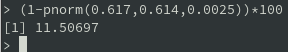
\includegraphics{tugas1b}\\
        probabiliatas kumulatif x dengan rata-rata $\lambda = 0,614$ atau $P(X > 0,617)$. Kita gunakan syntax pnorm(x, mean(rata-rata), standar deviasi). Kemudian kita masukkan dalam Rconsole seperti gambar dibawah yaitu  b = 1-pnorm(0.617,0.614,0.0025). Setelah itu kita kalikan dengan 100, maka akan muncul output seperti gambar dibawah ini. Jadi persentase banyaknya bantalan peluru yang memiliki massa lebih berat dari 0,617 adalah 11,5\%.
    \item kurang dari 0,608 kg\\
        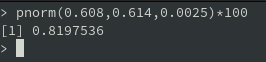
\includegraphics{tugas1c}\\
        Untuk mencari probabiliatas kumulatif x dengan rata-rata $\lambda = 0,624$ atau P(X < 0,608). Kita gunakan syntax  pnorm(x, mean(rata-rata), standar deviasi). Kemudian kita masukkan dalam Rconsole seperti gambar dibawah yaitu pnorm(0.608,0.614,0.0025). Selanjutnya klik enter pada keyboard maka akan muncul output seperti gambar dibawah ini. Jadi persentase banyaknya bantalan peluru yang memiliki massa kurang dari 0,608 kg adalah 0,8\%.
\end{enumerate}

\paragraph{Tugas 2\\}
Pipa api untuk broiler yang dimanufaktur oleh sebuah perusahaan memiliki daya tahan rata-rata 8000 jam pemakaian dengan deviasi standard 600 jam. Tentukan Probabilitas daya tahan pipa
\begin{enumerate}[label=\alph*.]
    \item antara 7900 dan 8100 jam\\
        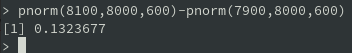
\includegraphics{tugas2a}\\
        Pada tugas ini kita akan menentukan probabilitas jika X 7900 sampai 8100 maka kita gunakan 2 perintah pada Rconsole. Untuk mencari probabiliatas kumulatif x dengan rata-rata $\lambda = 8000$ atau $P(7900 < X < 8100)$. Kita gunakan syntax pnorm(x, mean(rata-rata), standar deviasi). Kemudian kita masukkan dalam Rconsole seperti gambar dibawah yaitu pnorm(8100,8000,600)-pnorm(7900,8000,600). Maka akan muncul output seperti gambar dibawah ini. Jadi probabilitas daya tahan pipa antara 7900 sampai
        8100 jam $P(7900 < X < 8100)$ adalah 0,132.
    \item Kurang dari 7850 jam\\
        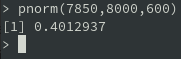
\includegraphics{tugas2b}\\
        Untuk mencari probabiliatas kumulatif x dengan rata-rata $\lambda = 8000$ atau $P(X < 7850)$. Kita gunakan syntax pnorm(x, mean(rata-rata), standar deviasi). Kemudian kita masukkan dalam Rconsole seperti gambar dibawah yaitu pnorm(7850,8000,600). Selanjutnya klik enter pada keyboard maka akan muncul output seperti gambar dibawah ini. Jadi probabilitas daya tahan pipa kurang dari 7850 jam adalah 0,401.
    \item Lebih dari 8200 jam\\
        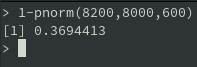
\includegraphics{tugas2c}\\
        Kemudian kita akan mencari probabiliatas kumulatif x dengan rata-rata $\lambda = 0,614$ atau $P(X > 8200)$. Kita gunakan syntax pnorm(x, mean(rata-rata), standar deviasi). Kemudian kita masukkan dalam Rconsole seperti gambar dibawah yaitu 1-pnorm(8200,8000,600). Setelah itu klik enter, maka akan muncul output seperti gambar dibawah ini. Jadi probabilitas daya tahan pipa lebih dari 8200 adalah 0,369.
\end{enumerate}

\newpage 
\section{Kesimpulan}
setelah praktikum lebih memahami tentang probabilitas diskrit kontinyu. Dan juga lebih memahami menghitung probabilitas pada distribusi normal dan student-t. Serta mampu membangkitkan data berdistribusi normal dan student-t.

\end{document}
